\section{Design of PID Controllers}

\subsection{P-controller}

The control law for the proportional controller is given by
$$ u(t) = K_p e(t) $$
where $K_p$ is the proportional gain and $e(t)$ is the error signal.

The controller applies a control signal to the systen,
which depends linearly on the error signal.

To eliminate the steady state error, feedforward
can be added to the P-controller.
$$ u(t) = K_p e(t) + u_{ff} $$

Where the term $u_{ff}$ is also called reset. We choose the feedforward
according to the DC gain of the system, i.e.
$$ u(t) = K_p e(t) + \frac{1}{G(0)} r(t) $$

The feedforward does not affect the poles of the closed loop system.

\subsection{PI-controller}

The control law of a proportional-integral feedback controller is given by:
$$u = K_p e + K_I \int_{t_0}^t e(\tau) d\tau$$
The controller adds a term, which is proportional to the integral of the error
e to the P-control term.

\begin{center}
	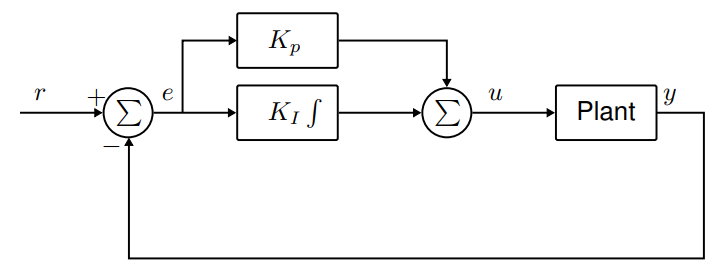
\includegraphics[width = 0.5\textwidth]{Images/PI-controller.png}
\end{center}

The purpose of adding the integral term is to
eliminate the steady state error of the system without the need for
feed forward, i.e., integral control is less sensitive to modelling errors.
Feed forward cannot eliminate modelling errors, but integral control can.

Comparing the PI-controller to the P-controller, the PI-controller has
a better response to disturbances, that are unknown or cannot be measured.
This is because the feedforward control can only eliminate the steady state error
if the model and disturbances are known.



Implementation of a PI-controller is called automatic reset, and is
shown in the following figure.


\begin{center}
	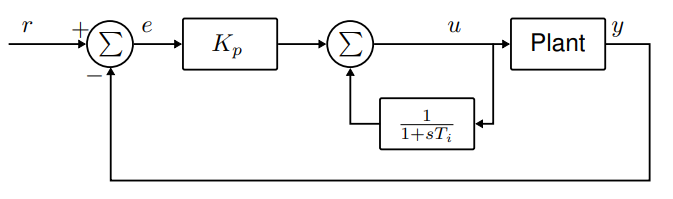
\includegraphics[width = 0.5\textwidth]{Images/PI-implementation.png}
\end{center}

On the figure, $T_i$ is the integration time (integraltid). The
transfer function from $e$ to $u$ is given by:
$$ T_{ue} = K_p \frac{1 + sT_i}{sT_i} = K_p + \frac{K_p}{sT_i} $$
\newpage
On the figure below the step respones are shown for $K_i = 0,0.2,0.5$ and $K_p = 1$
\begin{center}
	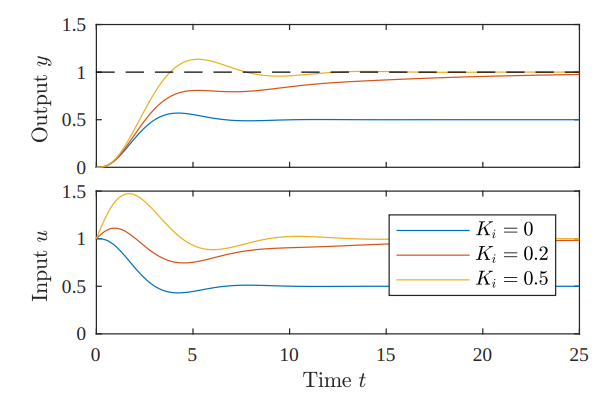
\includegraphics[width = 0.5\textwidth]{Images/PI-unitStep.png}
\end{center}
From the unit step response it can be seen that the integral action removes
the steady state error. A large $K_i$ will give a fast response, but also
a large overshoot. A small $K_i$ will give a slow response, but also a small
overshoot.


\subsection{PD-controller}
The derivative term provides an anticipatory action to the control,
by doing feedback based on the trend of the error, i.e.
$$u(t) = K_p e(t) + K_d \frac{de(t)}{dt} = K_p \left(e+T_d\frac{de(t)}{dt}\right)$$

Where $k_d$ is the derivative gain and $T_d$ is the derivative time constant and $e_p$
is a prediction of the error  ($T_d$ forwards in time). The parenthesis in the equation on the right
is a prediction of the error called $e_p$.

\textbf{PD-implementation}
\begin{center}
	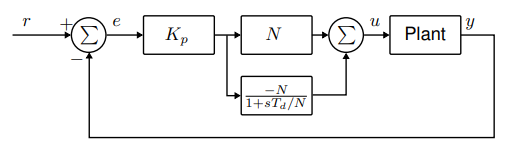
\includegraphics[width = 0.5\textwidth]{Images/PD-implementation.png}
\end{center}

Noise is an issue for controllers that include a derivative term. Therefore, they can
be implemented in a low-pass filtered version.

The transfer function of the controller is
$$T_{ue}(s) = K_p \left(N-\frac{N}{1+sT_d/N}\right) = K_p \frac{sT_d}{1+sT_d/N}$$

Where N is a filter constant (typical values of N are 2 to 20), and $T_d$ is the derivative time constant.

\newpage

The bode plot of an ideal PD-controller and a filtered PD controller are similar for low frequencies.
Using a low-pass filter, we can at a certain frequency, reduce the gain of the derivative term, and
thereby reduce the noise amplification.

\begin{center}
	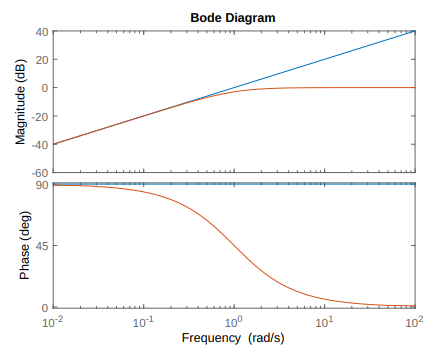
\includegraphics[width = 0.5\textwidth]{Images/bode-pd.png}
\end{center}

\subsection{PID-controller}
The control law of a PID feedback controller is
$$u(t) = K_p e(t) + K_i \int_{t_0}^t e(\tau) d\tau + K_d \frac{de(t)}{dt}$$

A block diagram of the controller is given below:
\begin{center}
	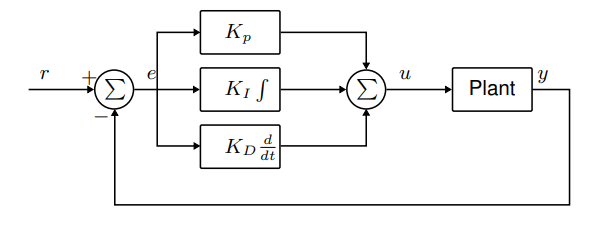
\includegraphics[width = 0.5\textwidth]{Images/pid.png}
\end{center}

Alternatively, the PID-controlelr with filter on the D-term is
$$K(s) = K_p \left(1+\frac{1}{T_i s} + \frac{sT_d}{1+sT_d/N}\right)$$

\subsection{Tuning a PID Controller}
\subsubsection{Pole placement}

If a model of the system is available, then it is possible to compute an expression
for the characteristic polynomial of the closed-loop system. Based on this polynomial,
it may be possible to place the poles at desired locations.

\subsubsection{Ziegler-Nichols method}

Sometimes a model of the plant is not availabe, then the controller should be tuned
by only studying the input-output behaviour of the system.
Ziegler and Nichols has proposed two methods for tuning PID controllers without
explicit use of a plant model.

\begin{itemize}
	\item{Ziegler-Nichols tuning based on step response}
	\item{Ziegler-Nichols tuning - The ultimate sensitivity method}
\end{itemize}


\textbf{Tuning based on step response}

The considered system is assumed to have the transfer function
$$\frac{y(s)}{u(s)} = \frac{A}{\tau s + 1} e^{-st_d}$$

This is a first-order system with a time delay of $t_d$.

The parameters for the PID controller can be found using the following table:
\begin{table}[h]
\centering
\begin{tabular}{|c|c|}
\hline
\cellcolor[HTML]{C0C0C0} \textbf{Controller type}& \cellcolor[HTML]{C0C0C0}\textbf{Gains}  \\ \hline
P&$K_p=\frac{1}{RL}$ \\ \hline
PI&$K_p=\frac{0.9}{RL}$\\
  &$T_i=\frac{L}{0.3}$\\ \hline
& $K_p=\frac{1.2}{RL}$ \\
 PID &$T_i=2L$ \\
  &$T_d=0.5L$\\ \hline
\end{tabular}
\end{table}

where $R=A/\tau$ is the amplitude of the oscillation, and $L$ is the period of the oscillation.

\textbf{The ultimate sensitivity method}

Start using a P-controller, and increase the gain until the system starts to oscillate.
The value of $K_p$ when the output oscillates with a constant amplitude is called the ultimate gain $K_u$.
The period of the oscillation is called the ultimate period $P_u$.

The parameters for the PID controller can be found using the following table:
\begin{table}[h]
\centering
\begin{tabular}{|c|c|}
\hline
\cellcolor[HTML]{C0C0C0} \textbf{Controller type}& \cellcolor[HTML]{C0C0C0}\textbf{Gains}  \\ \hline
P&$K_p=0.5K_u$ \\ \hline
PI&$K_p=0.45K_u$\\
  &$T_i=\frac{P_u}{1.2}$\\ \hline
& $K_p=0.6K_u$ \\
 PID &$T_i=0.5K_u$ \\
  &$T_d=\frac{1}{8}P_u$\\ \hline
\end{tabular}
\end{table}


\subsection{Examples}
